%%%%%%%%%%%%%%%%%%%%%%%%%%%%%%%%%%%%%%%%%%%%%%%%%%%%%%%%%%%%%%%%%%
%%%%%%%% ICML 2013 EXAMPLE LATEX SUBMISSION FILE %%%%%%%%%%%%%%%%%
%%%%%%%%%%%%%%%%%%%%%%%%%%%%%%%%%%%%%%%%%%%%%%%%%%%%%%%%%%%%%%%%%%

% Use the following line _only_ if you're still using LaTeX 2.09.
%\documentstyle[icml2013,epsf,natbib]{article}
% If you rely on Latex2e packages, like most moden people use this:
\documentclass{article}

% For figures
\usepackage{graphicx} % more modern
%\usepackage{epsfig} % less modern
\usepackage{subfigure} 

% For citations
\usepackage{natbib}

% For math
\usepackage{array}
\usepackage{amssymb}
\usepackage{amsmath}
\usepackage{amsthm}

% For algorithms
\usepackage{algorithm}
\usepackage{algorithmic}

% As of 2011, we use the hyperref package to produce hyperlinks in the
% resulting PDF.  If this breaks your system, please commend out the
% following usepackage line and replace \usepackage{icml2013} with
% \usepackage[nohyperref]{icml2013} above.
\usepackage{hyperref}

% Packages hyperref and algorithmic misbehave sometimes.  We can fix
% this with the following command.
\newcommand{\theHalgorithm}{\arabic{algorithm}}

\DeclareMathOperator*{\argmax}{arg\,max}

% Employ the following version of the ``usepackage'' statement for
% submitting the draft version of the paper for review.  This will set
% the note in the first column to ``Under review.  Do not distribute.''
% \usepackage{icml2013} 
% Employ this version of the ``usepackage'' statement after the paper has
% been accepted, when creating the final version.  This will set the
% note in the first column to ``Proceedings of the...''
\usepackage[accepted]{icml2013}


% The \icmltitle you define below is probably too long as a header.
% Therefore, a short form for the running title is supplied here:
\icmltitlerunning{Deep Belief Networks for Audio Chord Recognition}

\begin{document} 

\twocolumn[
\icmltitle{Deep Belief Networks for Audio Chord Recognition}

% It is OKAY to include author information, even for blind
% submissions: the style file will automatically remove it for you
% unless you've provided the [accepted] option to the icml2013
% package.
\icmlauthor{Benjamin Rapaport}{bar2150@columbia.edu}
\icmladdress{Columbia University,
            2960 Broadway  New York, NY 10027}
\icmlauthor{Samuel Messing}{sbm2158@columbia.edu}
\icmladdress{Columbia University,
            2960 Broadway  New York, NY 10027}

% You may provide any keywords that you 
% find helpful for describing your paper; these are used to populate 
% the "keywords" metadata in the PDF but will not be shown in the document
\icmlkeywords{deep learning, deep belief networks, hessian free, machine learning}

\vskip 0.3in
]

\begin{abstract}

Feature selection plays a critical role in audio analysis, with most Music
Information Retrieval (MIR) systems relying on a standard set of manually
crafted, domain-specific features. In this paper, we explore the possibility of
using Deep Belief Networks (DBNs) to discover better features through an
unsupervised training procedure as part of a chord-recognition system.
Specifically, we explore training DBNs using a number of methods including the
Contrastive Divergence algorithm, error backpropagation and a new technique
called Hessian-Free optimization. We evaluate the learned features by comparing
the performance of Structured Suport Vector Machines (StructSVMs) trained on
the DBN-learned features to StructSVMs trained on a standard human-engineered
feature set, called Chroma. We also explore the possibility of training DBNs to
perform chord-recognition directly.

\end{abstract} 

\section{Introduction}
\label{sec:intro}

The success and failure of many machine learning techniques is often strongly
influenced by the representations of data used for learning.  Historically,
this has motivated a large focus on feature engineering, wherein
domain-specific expertise and human ingenuity is used to design a series of
preprocessing steps to transform the original input data into a form that is
easy to learn from. Recently, with the advent of efficient algorithms for
training many-layered (deep) neural networks, researchers have begun to explore
using neural networks to learn a set of features directly from the data itself.
This process is often called "deep learning".

One of the most popular and successful methods for unsupervised feature
learning has been the use of Deep Belief Networks (DBN), a specific class of
neural networks, to learn a set of features that can then be used for
classification tasks. This technique has been used to achieve state-of-the-art
performance on a number of standard learning tasks across multiple modalities,
including speech recognition \cite{Mohamed_acousticmodeling, dahl2010phone},
polyphonic music transcription \cite{boulanger2012modeling}, and object
recognition \cite{krizhevsky2012imagenet, ciresan2012multi, rifai2011manifold}.

Interest in the use of neural networks for unsupervised feature learning has
increased in the last few years with the development of efficient training
algorithms \cite{Hinton06afast}. Research and evaluation of these algorithms
suggest that they enable the hidden layers of a network to pick up on
statistical relationships across many different levels of abstraction. It is
thought that the training algorithms also help networks to avoid bad local
minima and provide a better set of initial weights to be used with standard
error backpropagation training \cite{Bengio_learning}.

In this work, we investigate the use of Deep Belief Networks for automatically
learning a set of features for use in automatically identifying chords played
in songs. The task is somewhat simple: given a song, produce a list of
(timestamp, chord) labels to indicate which chords are played. We attempt to
accomplish this task in two ways. First, we explore using DBNs to learn a set
of features to use as input into a Structured Support Vector Machine, which is
capable of learning how to make structured predictions.  Second, we explore
using DBNs to label the chords of songs directly.

The paper is structured as follows: in \S \ref{sec:dataset}, we briefly cover
the input dataset as well as the human-engineered feature set which we will be
comparing our results to. In \S \ref{sec:DBN} we discuss the theory motivating
Deep Belief Networks and overview the algorithms we use to train them. \S
\ref{sec:svms} discusses the Structured Support Vector Machine model. In \S
\ref{sec:methods} we overview the different models and methods used in our
experiments. Lastly, in \S \ref{sec:results} we present the performance of our
models and compare them to models trained with human-engineered features
directly.


\section{Dataset} 
\label{sec:dataset}

The training and evaluation of our techniques was performed on a set of 180
hand-labeled Beatles songs \cite{harte2010towards}. The set of chord labels was
restricted to triads: 12 labels for each of the major triads (e.g. C major, D
major), 12 for each of the minor triads (e.g. C minor, D minor), and a final
label representing 'no chord', for a total of 25 possible chord labels.

\subsection{Chroma}

The first feature class we explored was Chroma, a human-engineered feature
class. To compute chroma, a song is first split into beat-synchronous frames.
For each frame, 12 features are computed, representing the intensity of each
semitone of the Western music scale, irrespective of octave. Each of these
features is constrained to be in the range [0,1].

\subsection{Short-Time Fourier Transform}

In addition to the human-engineered chroma features, we investigated the
performance of both DBNs and StructSVMs on raw audio input. To transform a raw
audio signal into a convenient format for our models, we took the following
preprocessing steps: First, the raw audio signal of each song was downsampled
to 44kHz. Second, a Short-Time Fourier Transform (STFT) was performed with a
hamming window of 186ms (8192 samples) with a 50\% overlap between windows. The
transform was computed for 1024 frequencies, of which we only kept the absolute
values and thus considering the symmetry of the FT were left with 512
frequencies. As a final preprocessing step, Principal Component Analysis (PCA)
whitening was applied to the spectrograms to further reduce the dimensionality
(using 256 components) of our input data and make the variance
spherical.\footnote{The testing dataset was always left out of the
  calculations required for PCA whitening, including the calculation of the
centroid vector and whitening matrix.  Instead these were calculated using only
the training set. The test data were then whitened using the pre-generated
centroid vector and whitening matrix.}

\begin{figure}[ht]
\vskip 0.2in
\begin{center}
\centerline{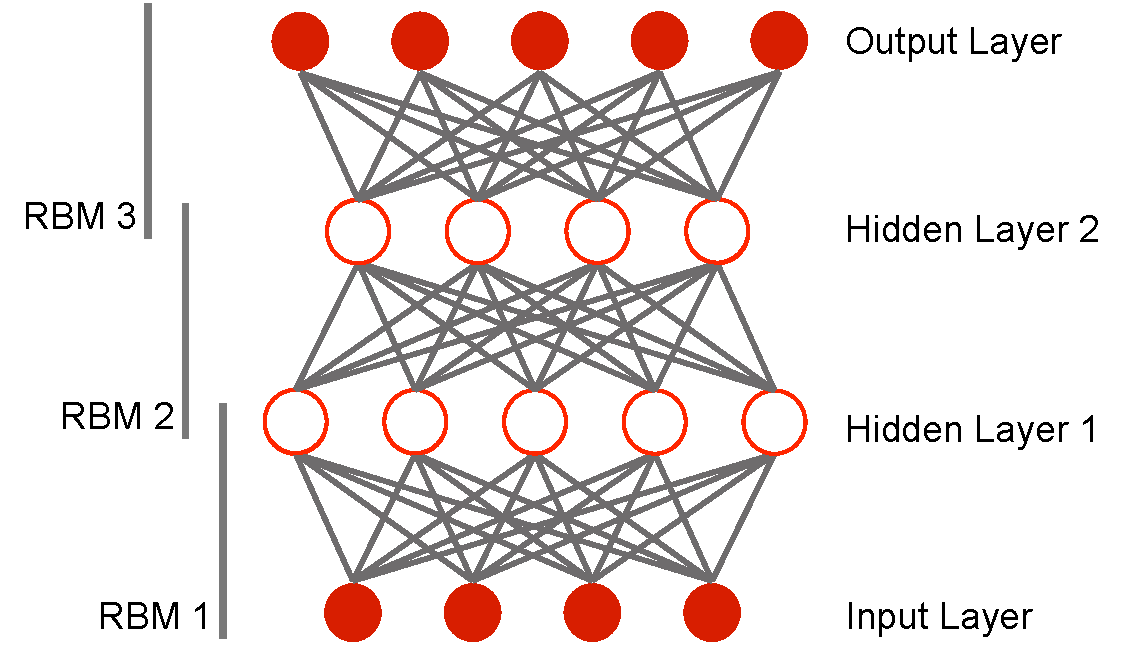
\includegraphics[width=\columnwidth]{images/deep_network_arch.pdf}}
\caption{The general architecture of a DBN as a series of stacked RBMs}
\label{dbn-arch}
\end{center}
\vskip -0.2in
\end{figure}

\section{Deep Belief Networks}
\label{sec:DBN}

\subsection{Restricted Boltzmann Machines}

The main building block of a Deep Belief Network is the Restricted Boltzmann
Machine (RBM). An RBM is an undirected graphical model defining a joint
probability distribution over a vector of observed variables, $\mathbf{v}$ and
a vector of hidden variables, $\mathbf{h}$ \cite{mnih2012conditional}. The RBM
is a bipartite graph, where each visible node is connected to every hidden
node, but no other visible nodes, and vice versa for the hidden nodes. This
allows for both $p(\mathbf{h}|\mathbf{v})$ and $p(\mathbf{v}|\mathbf{h})$ to
factor over the variables, allowing inference to be computed efficiently while
avoiding the ``explaining away'' phenomenon (the set of visible or hidden
variables are independent of each other given the other set). Assuming each of
these vectors is binary, the RBM models the joint probability distribution

\[
  p \left( \mathbf{v}, \mathbf{h} \right) = 
  \exp \left(\dfrac{-E \left( \mathbf{v}, \mathbf{h} \right)}{Z}\right),
\]

where $Z$ is the normalization term, and $E$ is an energy function defined as

\[
  E \left( \mathbf{v}, \mathbf{h} \right) = 
  - \mathbf{v^TWh} - \mathbf{v^Tb^v} - \mathbf{h^Tb^h}.
\]

$\mathbf{W}$ is a matrix of pairwise weights between the elements in 
$\mathbf{v}$ and $\mathbf{h}$, $\mathbf{b^v}$ are the biases for the visible
vector elements, and $\mathbf{b^h}$ are the biases for the hidden vector
elements.

If we define the free energy $F(\mathbf{v})$ as
\begin{align*}
  F \left( \mathbf{v} \right) &= -\log \sum_{\mathbf{h}} \exp \left( -E \left( \mathbf{v,h} \right) \right) \\
  &= \mathbf{v^Tb^v} - \sum_{\mathbf{j}} \log
    \left(
      1 + \exp \left( b_j^h + \mathbf{v^TW_{\cdot j}} \right)
    \right), \\
\end{align*}

then we can obtain the distribution $p(\mathbf{v})$ by marginalizing over
$\mathbf{h}$

\begin{align*}
  p(\mathbf{v}) &= \dfrac{\sum_{\mathbf{h}} \exp(-E(\mathbf{v, h}))}{Z} \\
                &= \dfrac{\exp(-F(\mathbf{v}))}{Z}. \\
\end{align*}

An RBM can be trained using gradient descent of the negative
log-likelihood, where the log-likelihood is defined as:

\begin{align*}
  l(\theta) &= \log \, p(\mathbf{v}) \\
            &= -F(\mathbf{v}) - \log \sum_{\mathbf{v'}} \exp \left(-F(\mathbf{v'})\right), \\
\end{align*}

which yields the following gradient,

\begin{equation}
  \label{eq:rbm:grad}
  \frac{- \partial l(\theta)}{\partial \theta}
  = \frac{\partial F(\mathbf{v})}{\partial \theta} - 
  \sum_{\mathbf{v'}}\frac{\partial F(\mathbf{v'})}{\partial \theta}
                  p(\mathbf{v})
\end{equation}

While this method works in theory, Equation \ref{eq:rbm:grad} is intractable to
compute for all but the smallest of models, as the second term on the
right-hand side is an expectation over the model distribution $p(\mathbf{v})$.


\subsection{Contrastive Divergence}

In 2002, Geoff Hinton introduced an efficient method for training RMBs called
Contrastive Divergence \cite{hinton_contrastivedivergence, Hinton06afast}. In
this method, we calculate the derivative of the log probability for a particular
training vector with respect to a given weight vector $\mathbf{W}$ as,

\begin{equation}
  \label{eq:cd}
  \frac{\partial \log p(\mathbf{v})}{\partial w_{ij}} = 
  \langle v_i h_j \rangle_{data} - \langle v_i h_j \rangle_{model},
\end{equation}

where the angle brackets indicate expectations under the specified
distributions.  Because the RBM is bipartite, obtaining samples from the hidden
units given visible activations can be accomplished using the following
equation,

\[
  p (h_j = 1 | \mathbf{v}) = \sigma\left(b_{j}^{h} + \sum_i v_{i} w_{ij}\right),
\]

where $\sigma$ is the logistic sigmoid function. To obtain samples for the
visible units given hidden activations, we make a similar computation,

\[
  p (v_i = 1 | \mathbf{h}) = \sigma\left(b_{i}^{v} + \sum_j h_j w_{ij}\right).
\]


If the visible units are real-valued instead of binary, we can use a
Gaussian-Bernoulli RBM by simply changing the sampling equation for the visible
vector to be:
\[
  p (v_i | \mathbf{h}) = \mathcal{N} \left( b_{i}^{v} +
    \sigma_i \sum_j h_j w_{ij} \,,\, \sigma_i^2 \right),
\]

where we generally normalize the data such that $\sigma = 1$.

We could compute the expectation under the model by running a Gibbs chain for a
long time, where we alternatively sample hidden states given visible states,
and visible states given hidden states repeatedly until we converged on the
model distribution. However, the insight of Contrastive Divergence is that if
we initialize the visible vector by clamping it to a training vector sampled
from the empirical data distribution, and only take a few Gibbs sampling steps,
we can obtain an estimate of the model distribution called the
``reconstruction'' that works well empirically for estimating the gradient. In
fact, good results can be obtained by taking a single Gibbs step.  The learning
rule for updating a weight between two units with learning rate $\eta$ is then

\[
  \triangle w_{ij} = \eta( 
  \langle v_i h_j \rangle_{data} - \langle v_i h_j \rangle_{recon}
  )
\]

which as opposed to Equation \ref{eq:rbm:grad} can be computed efficiently for
all sizes of RBMs.

\subsection{Training a DBN with Contrastive Divergence and Supervised Fine-Tuning}

We can construct an arbitrarily deep neural network by stacking a series of
RBMs on top of each other. To train the DBN, we train each one of the stacked
RBMs individually using the Contrastive Divergence (CD) technique. Starting at
with the bottommost visible layer, we train successive layers in a bottom-up
fashion, using the hidden layer of the previous layer's RBM as the visible
layer for the RBM above it (we initialize the visible vector of the first layer
using our input data). Each RBM is trained by sampling from the distributions
below it to initialize the visible vectors for CD training.

Once each layer has been trained, the final step for training the DBN is to
unfold its layers into a standard, feed-forward neural network, and add a final
softmax layer of output units that can be used for classification. We use the
weights learned from the unsupervised CD pre-training to initialize the weights
of the feed forward network, which are then fine-tuned in a supervised manner
using error backpropagation on a set of labeled examples. It is thought that
the unsupervised pre-training helps to find a good initialization of the weights
of the feed-forward network by avoiding local minima \cite{Bengio:2009:LDA}.

\subsection{Training a Deep Neural Network with Hessian Free Optimization}

Recently, Martens has proposed an alternative approach to the one presented
above that can achieve similar performance and requires no pre-training
\cite{martens2010deep}.  As opposed to traditional error backpropagation, this
technique relies on a second-order method called Hessian-Free (HF)
optimization. Using HF, Martens was able to obtain similar and sometimes
superior results for training deep networks than the methods described above.

Second-order optimization techniques can be more effective than normal gradient
descent methods because they take into account information about the local
curvature of the objective function when performing parameter updates. This
additional information allows these techniques to avoid the trappings of
pathological curvature in the parameter space, which has been known for some
time to be a major issue with training deep neural networks. By taking
second-order information into account, these learning methods also have fewer
adjustable parameters than traditional first-order methods, as details such as
the step size for a particular update can be computed using a line search,
rather than being defined by a fixed constant.

HF techniques belong to the class of approximate Newton methods for the
minimization of real-valued, smooth-objective functions
\cite{martens2012training}. The basic idea behind HF is derived from Newton's
method, where local quadratic approximations of the objective function are
iteratively optimized to produce updates to the parameters $\mathbf{\theta}$.
More precisely, at each step we optimize a local quadratic model
$M_{k-1}(\mathbf{\delta)}$ of the objective function $f(\mathbf{\theta_{k-1}} +
\mathbf{\delta})$, which is estimated using the gradient and curvature
information local to $\mathbf{\theta_{k-1}}$, to produce a new parameter vector
$\mathbf{\theta_k}$. The quadratic approximation is defined as,

\[
  M_{k-1}(\mathbf{\delta}) = f(\mathbf{\theta}_{k-1})
  + \nabla f(\mathbf{\theta_{k-1})^T \delta}
  + \frac{1}{2} \mathbf{\delta^T B_{k-1} \delta},
\]

where $\mathbf{B_{k-1}}$ is the curvature matrix, which is the Hessian
$\mathbf{H(\theta_{k-1})}$ of $f$ at $\mathbf{\theta_{k-1}}$ for Newton's
method. The updated parameters are then computed as $\mathbf{\theta_{k-1}} +
\alpha_k \mathbf{\delta^{*}_{k}}$, where $\mathbf{\delta^{*}_{k}}$ is the
minimizer of $M_{k-1}(\mathbf{\delta)}$ and $\alpha_k$ is the step-size chosen
via line search.

When the curvature matrix $\mathbf{B_{k-1}}$ is positive definite, the
minimizer will exist and is given by

\[
  \mathbf{\delta^{*}_{k}} =
  \mathbf{\theta_k} - \mathbf{B^{-1}_{k-1}} \nabla f(\mathbf{\theta_{k-1}}).
\]


For neural networks, it is intractable to compute the Hessian of the objective
function directly as the matrix is $\mathcal{O}(n^2)$ in the number of
parameters, $n$. In addition to calculating the Hessian, inverting the matrix
in order to solve for the minimizer is even more costly, requiring
$\mathcal{O}(n^3)$ computations. To avoid computing and inverting the Hessian,
HF and other so-called truncated Newton methods approximately optimize the
quadratic function $M$ using the conjugate gradient (CG) algorithm to update
$\theta$ at each step. This alternative is efficient because CG only requires
matrix-vector products with the curvature matrix $\mathbf{B}$, which can be
computed efficiently.

For the full mathematic and technical details of the HF method, see
\cite{martens2012training}.

\section{Large Margin Structured Predictions}
\label{sec:svms}

Finally, to make predictions for the sequence of chord labels over a song,
we turn to an extension of Support Vector Machines (SVM) that can support
structured classification problems such as sequence prediction. Under this
extension, the goal is to learn a function $F : X \times Y \rightarrow
\mathbf{R}$ with weight vector $\mathbf{w}$ such that,

\begin{equation*}
f(\mathbf{x}) = \argmax_{y \in Y}F(\mathbf{x},\mathbf{y}\,;\,\mathbf{w})
\end{equation*}

correctly predicts the true label $y$. Given a series of $N$ data points
$(\mathbf{x}^{(i)}, \mathbf{y}^{(i)})_{i=1}^{N}$, we can learn the weight
vector $\mathbf{w}$ by imposing data-specific constraints of the following
form,

\begin{equation*}
\begin{split}
F(\mathbf{x}^{(i)}, \mathbf{y}^{(i)}\,;\,\mathbf{w}) -
F(\mathbf{x}^{(i)}, \mathbf{y}'\,;\,\mathbf{w}) \geq 1 \\
\forall i \in 1\dots N,\,\mathbf{y}' \neq \mathbf{y}^{(i)}
\end{split}
\end{equation*}

Learning is accomplished by minimizing $||\mathbf{w}||$ subject to the
data-specific constraints. The optimization problem is thus,

\[
\begin{split}
\min_{\mathbf{w}}\dfrac{1}{2}||\mathbf{w}||\quad\text{such that,} \\
F(\mathbf{x}^{(i)}, \mathbf{y}^{(i)}\,;\,\mathbf{w}) -
F(\mathbf{x}^{(i)}, \mathbf{y}'\,;\,\mathbf{w}) \geq 1 \\
\forall i \in 1\dots N, \,\mathbf{y}' \neq \mathbf{y}^{(i)}
\end{split}
\]

When data is non-separable, additional slack variables are introduced to allow
for a certain amount of disagreement between the predicted and true labels.
  This enables the learning algorithm to effectively ignore hard-to-label
  points. With the added $N$ slack variables, $\xi$, the optimization problem
  becomes,

\begin{align*}
\begin{split}
\min_{\mathbf{w, \xi}}\dfrac{1}{2}||\mathbf{w}|| +
\dfrac{C}{N}\sum_{i=1}^{N}\xi^{(i)}
\quad\text{such that,}&\\
F(\mathbf{x}^{(i)}, \mathbf{y}^{(i)}\,;\,\mathbf{w}) -
F(\mathbf{x}^{(i)}, \mathbf{y}'\,;\,\mathbf{w}) \geq 1 - \xi^{(i)} \\
\forall i \in 1\dots N, \,\mathbf{y}' \neq \mathbf{y}^{(i)}
\end{split}
\end{align*}

Where $C$ is a tunable parameter that represents the cost associated with
using slack. When $C = \infty$, the optimization problem is the same as in
the separable case.

For sequence learning, the class $Y$ of possible labellings can be exponential
in size, and therefore it is often infeasible to enumerate all of the
data-specific constraints. Instead, the SVM$^{struct}$ algorithm uses an
efficient cutting-plane approach to find a solution after adding only a
polynomial number of constraints. This involves reformulating the problem from
an $N$-slack problem ($N$ $\xi$ variables) to a 1-slack problem (only a single
$\xi$ variable). This reformulation only requires that the calculation of
$\hat{y} = \argmax_{y \in Y}$ be efficiently computable for all examples. The
details can be found in \cite{joachims2009cutting}.

\subsection{The SVM$^{hmm}$ model}

The SVM$^{hmm}$ model is a particular formulation of SVM$^{struct}$ where the
discriminant function is constructed to be isomorphic to a $k$th order Hidden
Markov Model (HMM). This model was first described in \cite{altun2003hidden}.
While this model does not have the same probabilistic interpretation as the
HMM, by mimicking the structure of a traditional HMM, $\argmax_{y \in Y}$
becomes efficient to compute, as the same Markov property\footnote{Again, we
  stress that in the case of SVM$^{hmm}$ there is no probabilistic
interpretation, we use the term ``Markov property'' loosely.} can be exploited,
simplifying the algorithm. This enables the use of the cutting-plane method
mentioned above..

To mimic a $k$th order HMM, the function $F$ used by SVM$^{hmm}$ is of the
form,

\begin{flalign*}
  &{F(\mathbf{x}, \mathbf{y}\,;\,\mathbf{w})} =& \\
    & \sum_{t=1}^{T} \left[
      \sum_{k=1}^{K}\left(
        \mathbf{x}_{t} \cdot
        \mathbf{w}_{\mathbf{y}_{(t-k)} \dotsm \mathbf{y}_{t}} +
        \phi_{\text{trans}}(y_{(t-k)},\dots,y_{t}) \cdot
        \mathbf{w}_{\text{trans}}
      \right)
    \right]  &
\end{flalign*}

Where $T$ is the number of time frames in an individual example ($\mathbf{x}$,
$\mathbf{y}$), $x_t$ is the $t^{\text{th}}$ frame of example $x$, $K$ is the
order of dependencies, and $\phi_{\text{trans}}$ is an indicator vector that
has exactly one entry 'on' (equal to 1) and all others 'off' (equal to 0),
corresponding to the sequence $(y_{(t-k)},\dots,y_{t})$.

\section{Methods}
\label{sec:methods}

For all of our models, we experimented with using both Chroma and raw STFTs
as the input data. We also experimented with concatenating surrounding frames
of each input vector we wanted to classify to give more contextual information
to the models.

We trained deep belief networks using either Contrastive Divergence (CD)
unsupervised pre-training followed by supervised error backpropagation, or
using the Hessian Free (HF) technique with no pre-training. For CD learning, we
made use of a library provided by Rasmus Berg Palm \cite{IMM2012-06284}. For
the HF technique, we used a library provided by Martens \cite{martens2010deep}.

After training, the test data was then either classified directly by the output
layer of the trained network, or was used to compute network activations which
were then fed into the structured SVM classifier \cite{joachims1999making}. For
every experiment, 5 random permutations of the songs were used for training,
with 10\% of the total song corpus reserved for training, and 10\% used as a
validation set to decide when to stop network training. All results reported,
unless specified otherwise, are an average of models trained on each of these 5
permutations.

\section{Results}
\label{sec:results}

\subsection{DBN with CD Pre-training Softmax Performance}

The first thing we attempted was to train DBNs using the standard Contrastive
Divergence approach discussed above. We focused on getting models to be
performant at predicting chord labels for individual frames alone. Based on
preliminary results, we trained a set of models on both Chroma and raw STFTs
using similar architectures.  Average performance results are presented in
Figure \ref{fig:dbn:softmax}, and correspond to 10 individual models trained on
10 differnt permutations of the Beatles set. All models were trained on 30\% of
the training data. The most performant of these models achieved an average
accuracy of 42.3\% at test.

\begin{figure*}
\begin{center}
\begin{tabular}{c|c|l}
Input & Structure & Acc. (avg.) \\
\hline
Chroma & 12$\rightarrow$50$\rightarrow$25$\rightarrow$25 & 39.36\% ($\pm$ 2.25) \\
Chroma & 12$\rightarrow$300$\rightarrow$300$\rightarrow$25 & 14.20\% ($\pm$ 1.42) \\
STFTs & 513 $\rightarrow$50$\rightarrow$25$\rightarrow$25 & 32.11\% ($\pm$ 1.55) \\
STFTs & 513 $\rightarrow$300$\rightarrow$300$\rightarrow$25 & 42.30\% ($\pm$ 2.6) \\
\end{tabular}
\label{fig:dbn:softmax}
\end{center}

\caption{Average softmax prediction accuracy for DBNs trained on 30\% of the
training data using CD pre-training and error backpropagation fine-tuning.
Results were calculated by training and evaluating individual models on 10
different permutations of the training data.}

\end{figure*}

Next, we trained another set of models using larger layers sizes since this
seemed to help networks do better. For this second set of models, we trained
networks with 80\% of the training set instead of 30\%. In addition, we
concatenated a number of previous and future frames to the input data to add
more temporal context. For Chroma networks, we included the four consecutive
previous and four consecutive future frames. For STFT networks, because the
original size is much larger, we concatenated just the previous two frames.
Figure \ref{fig:dbn:softmax:2} shows averaged results for these models. The
best network from this set achieved an average accuracy of 55.9\% at test, a
large improvement over the first set.


\begin{figure*}
  \begin{center}
\begin{tabular}{c|c|l}
Input & Structure & Acc (avg.) \\
\hline
Chroma & 108$\rightarrow$800$\rightarrow$600$\rightarrow$50$\rightarrow$25 & 46.2\% ($\pm$ 2.34) \\
Chroma & 108$\rightarrow$100$\rightarrow$100$\rightarrow$50$\rightarrow$25  & 55.9\% ($\pm$ 2.05) \\
STFTs & 768$\rightarrow$300$\rightarrow$200$\rightarrow$100$\rightarrow$25 & 48.8\% ($\pm$ 2.6) \\
STFTs & 768$\rightarrow$300$\rightarrow$300$\rightarrow$50$\rightarrow$25 & 42.8\% ($\pm$ 3.1) \\
\end{tabular}
\label{fig:dbn:softmax:2}
\end{center}

\caption{Average softmax prediction accuracy for DBNs trained on 80\% of the
  training data using CD pre-training and error backpropagation fine-tuning.
  For models trained on chroma, the 4 consecutive previous and 4 consecutive
  future frames were append to each individual frame to provide models with
more temporal context.  For models trained on raw STFTs, the 2 consecutive
previous frames were appended. Results were calculated by training and
evaluating individual models on 5 different permutations of the training data.}

\end{figure*}


\subsection{SVM Performance}

\begin{figure}
  \begin{center}
  \begin{tabular}{c|c|c|c}
    Layers & $C$ & $\epsilon$ & Avg. Accuracy \\
    \hline
    Chroma & 100 & 0.1 & 60.5\% ($\pm$ 2.6) \\
    All Layers & 10 & 0.5 & 57.6\% ($\pm$ 2.0) \\
  \end{tabular}
  \end{center}
  \caption{Average results for Support Vector Machines (SVMs) trained on
    Chroma-features and on DBN activations. All SVMs were trained on 30\% of
    the data set.}
  \label{fig:svms}
\end{figure}

Figure \ref{fig:svms} compares the average performance of SVMs trained on the
Chroma features directly to SVMs trained on the activations of a DBN previously
trained on the Chroma features. The network structure used for the DBN was
input\_layer $\rightarrow$ 100 $\rightarrow$ 100 $\rightarrow$ 50 $\rightarrow$
25. These networks were trained on 80\% of the Beatles data set. The SVMs
trained on DBN activations were outperformed by SVMs trained on the Chroma
features directly.  The average accuracy for SVMs trained on DBN activations
was 57.6\%, while the average accuracy of SVMs trained on Chroma features was
60.5\%. While less performant, the SVMs trained on DBN activations still
outperformed the original DBN softmax prediction accuracy, which for this
network as 55.9\%.

We attempted to also collect data for SVMs trained on the raw STFTs, but had
not anticipated the dramatic increase in training time required. While the
Chroma feature set breaks songs into approximately 200-300 frames of 12
features each, our STFT preprocessing generated on average 1000-2000
frames per song, with 256 features per frame. In order to reduce the training
time, we had to relaxed our original target goals for $C$ values as well as
$\epsilon$, but it wasn't enough to generated a full set of averaged results
within the time limit for this paper. However, individual results were in-line
with the results of SVMs trained on Chroma features and Chroma-trained DBN
activations.


\subsection{Deep Network Softmax Performance with HF training}

With the limited performance of DBNs trained with Contrastive Divergence and
the poor running time of the SVMs, we lastly turned our attention to the
Hessian-Free technique for training Deep Networks. This last technique resulted
in a dramatic increase in performance over our previous techniques. The results
reported in \ref{fig:hf:softmax} are average performances over 5 random
permutations of the training and testing data. Specifically, for each
permutation, 80\% of the songs were used to train the network, 10\% was used
as validation for choosing when to stop training as to avoid overfitting, 
and the final 10\% was used for testing.

The best performace was on a network trained on Chroma features, where inputs
included 6 frames to the left and 2 frames to the right of the center frame to
be labeled. The network architecture was input\_layer $\rightarrow$ 800
$\rightarrow$ 600 $\rightarrow$ 50 $\rightarrow$ 25, and resulted in
a classification accuracy of 65.60\%. Results for training on STFTs are also
reported, though the accuracy achieved on these features was significantly
lower.

We found that compared to the CD training, HF training was faster, less prone
to overfitting, and generally led to better results on the test sets.

\begin{figure*}
  \begin{center}
\begin{tabular}{c|c|l}
Input & Structure & Acc. (avg.) \\
\hline
Chroma L6R2 & 108$\rightarrow$300$\rightarrow$200$\rightarrow$100$\rightarrow$25 & 65.46\% ($\pm$ 1.67) \\
Chroma L6R2 & 108$\rightarrow$800$\rightarrow$600$\rightarrow$50$\rightarrow$25 & 65.60\% ($\pm$ 2.10) \\
STFT L2R0 & 1539$\rightarrow$300$\rightarrow$200$\rightarrow$100$\rightarrow$25 & 49.38\% ($\pm$ 1.85) \\
STFT L2R0 & 1539$\rightarrow$800$\rightarrow$600$\rightarrow$50$\rightarrow$25 & 50.37\% ($\pm$ 2.51) \\
\end{tabular}
\label{fig:hf:softmax}
\end{center}
\caption{
  Average softmax prediction accuracy for Deep Neural Networks trained with the
  Hessian Free method on 80\% of the training data. L and R values represent
  frames included from the left and the right of each center window as input to
  the network. A validation set of 10\% of the data was used to determine when
  to stop training in order to avoid overfitting. The final 10\% was used for
  testing.
}

\end{figure*}

\section{Future Work}
\label{sec:future_work}

Moving forward, the most natural extension of the work presented here would be
to train Recurrent Neural Networks (RNN) using the Hessian-Free method. RNNs
are similar to DBNs except each layer receives activation both from the layer
below it, and an additional layer which corresponds to the activation of the
particular layer at the previous time step. Neural networks constructed in this
way include a natural temporal element, which enables the networks to be much
more adept at structured prediction problems. We anticipate that this extension
would improve on the best models presented here.

In addition, given more time, it would be interesting to train networks using
the Contrastive Divergence method on a much larger training set than the
Beatles data set. Most state-of-the-art results involving Contrastive
Divergence required training networks on hundreds of thousands (and sometimes
millions) of unlabeled examples. We anticipate that doing the same thing in
this context may lead to a dramatic increase in performance of our DBNs, as the
additional unlabeled data will help the DBNs to generalize correctly.

\newpage

\bibliography{deep_belief_nets}
\bibliographystyle{icml2013}

\end{document} 


% This document was modified from the file originally made available by
% Pat Langley and Andrea Danyluk for ICML-2K. This version was
% created by Lise Getoor and Tobias Scheffer, it was slightly modified  
% from the 2010 version by Thorsten Joachims & Johannes Fuernkranz, 
% slightly modified from the 2009 version by Kiri Wagstaff and 
% Sam Roweis's 2008 version, which is slightly modified from 
% Prasad Tadepalli's 2007 version which is a lightly 
% changed version of the previous year's version by Andrew Moore, 
% which was in turn edited from those of Kristian Kersting and 
% Codrina Lauth. Alex Smola contributed to the algorithmic style files.  
